%! TEX root = ../listas_completas.tex

%%%%%%%%%%%%%%
%  EQUAÇÕES  %
%%%%%%%%%%%%%%

\section{Equações:}% \label{sec:equacoes_}
\begin{equation}\label{eq:zeta}
\zeta=\frac{c}{c_{c}}
\end{equation}
\begin{equation}\label{eq:Cc}
c_{c}=2 m \sqrt{\frac{k}{m}}=2 \sqrt{k m}=2 m \omega_{n}
\end{equation}
\begin{equation}\label{eq:xt}
    x_{t}=A_{1} e^{\lambda_{1} t}+A_{2} e^{\lambda_{2} t}
\end{equation}
Em que $\lambda_1$ e $\lambda_2$ são calculados com a equação~\ref{eq:lambda}
abaixo:
\begin{equation}\label{eq:lambda}
\lambda_{1,2}=\omega_{n}\left(-\zeta\pm \sqrt{\zeta^{2}-1}\right)
\end{equation}
Ou ainda da forma expandida:
\begin{equation}\label{eq:xt_expandida}
x_{t}=A_{1} e^{\left[\omega_{n}(-\zeta+\sqrt{\zeta^{2}-1})\right] t}+A_{2} e^{\left[\omega_{n}(-\zeta-\sqrt{\zeta^{2}-1})\right] t}
\end{equation}

\begin{itemize}
    \item Sistema Superamortecido: $\zeta > 1$
    \item Sistema criticamente amortecido: $\zeta = 1$
    \item Sistema sub-amortecido: $\zeta < 1$
\end{itemize}

%%%%%%%%%%%%%
%  Questão  %
%%%%%%%%%%%%%

\section{Lista 6}
\subsection{Questão 3.9}
A massa do sistema mostrado na figura é liberada a partir do repouso em $x_0 =
\SI{125}{mm}$, quando t=0. Determine o deslocamento $x $ em $t=\SI{0,65}{s}$ se
$c=\SI{300}{\newton\second\per\meter}$.
\begin{figure}[ht]
    \centering
    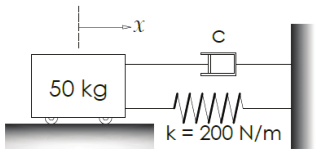
\includegraphics[width=0.3\textwidth]{imagens/questao_3.9.png}
    %\caption{}
    \label{fig:questao_3_9}
\end{figure}

%%%%%%%%%%%%%%%
%  Resolução  %
%%%%%%%%%%%%%%%

\resol

Cálculo de $c_c$ e $\zeta$:

Substituindo a equação (\ref{eq:Cc}) em (\ref{eq:zeta}), temos:
\[
\zeta = \frac{c}{2\cdot \sqrt{k\cdot m}} = \frac{300}{2\cdot \sqrt{200\cdot 50}} = 1,5
\]
$\zeta > 1$ constitui um sistema supercrítico.

Cálculo de $\omega_n$:
\[
\omega_n = \sqrt{\frac{k}{m}} = \sqrt{\frac{200}{50}} =
\SI{2}{\radian\per\second}
\]
Cálculo de $\lambda_1$ e $\lambda_2$:
da equação \ref{eq:lambda}, temos:
\[
    \lambda_1 = 2\cdot (-1,5 + \sqrt{1,5^2-1}) = -0,76
\]
\[
    \lambda_2 = 2\cdot (-1,5 - \sqrt{1,5^2-1}) = -5,23
\]
Temos então a equação \ref{eq:xt} na forma:
\[
x_t = A_1 e^{-0,76 t} + A_2 e^{-5,23 t}
\]
Encontrar os valores de $A_1$ e $A_2$:

Derivando $x_t$, obtemos a equação da velocidade $\dot x_t$:
\[
\dot x_t = -0,76 A_1 e^{-0,76 t}  -5,23 A_2 e^{-5,23 t}
\]
Substituindo $t=0$ na equação da posição, temos:
\[
x_0 = A_1 e^{0} + A_2 e^{0} \to x_0 = A_1 + A_2
\]
Do enunciado, temos que $x_0 = \SI{125}{mm}$, obtendo
\[
\SI{125}{mm} = A_1 + A_2
\]
Substituindo $t=0$ na equação da velocidade:
\[
\dot x_0 = -0,76A_1 - 5,23A_2 = 0
\]
Como a velocidade $\dot x_0 = 0$ no instante $t=0$, temos:
 \[
 0,76A_1 = 5,23A_2 \to A_1 = -6,88A_2
 \]
 Com isso, podemos substituir $A_1$ na equação da posição, obtendo:
\[
125 = -6,88A_2 + A_2 \to A_2 = \SI{-21,26}{mm}
\]
Com $A_2$ determinado, encontramos $A_1$ substituindo em $125 = A_1 + A_2$:
\[
    A_1 = 125 - (-21,26) \to A_1 = \SI{146,26}{mm}
\]
A equação da posição completa será então:
\[
x_t = 146,26 e^{-0,76 t} - 21,26 e^{-5,23 t}
\]
%E a equação da velocidade completa será:
%\[
    %\dot x_t = -0,76\cdot 146,26 \cdot e^{-0,76t} - 5,23 \cdot (-21,26)e^{-5,23 t}
%\]
Para $t=\SI{0,65}{s}$, temos:
\[
    x_{0,65} = 146,26 e^{-0,76 \cdot 0,65} - 21,26 e^{-5,23\cdot 0,65}
\]
\[
x_{0,65} = \SI{88,53}{mm}
\]
